%%%%%%%%%%%%%%%%%%%%%%%%%%%%%%%%%%%%%%%%%%%%%%%%%%%%%%%%%%%%%%%%%%
%%%%%%%%%%%%%%%%%%%%%%%%%%%%%%%%%%%%%%%%%%%%%%%%%%%%%%%%%%%%%%%%%%

\subsection{Ports}
Un processeur \acrshort{IA-32} a la possibilité de transférer des données en utilisant
les ports d'entrée/sortie. Ces ports sont utilisés par le processeurs pour communiquer
avec des périphériques. Il peuvent être utilisés pour envoyer et recevoir des données
(par exemple un \textit{timer} va utiliser les ports d'entrée/sortie pour envoyer
son état). Les ports peuvent aussi être utilisés pour contrôler un péripéhrique
à partir de registres de contrôle (par exemple avec un controlleur de disque).\cite{ref64}
Etant donné que nous ne sommes pas sur du vrai \textit{hardware}, QEMU va se charger
d'émuler les différents périphériques utilisés par un processeur Intel 32-bits. \\

Les ports d'entrées/sorties sur architecture x86 se situent dans un espace d'adresses
séparé de la mémoire physique. Cet espace permet d'adresser 64000 (soit $2^{16}$)
ports de 8 bits. Les ports sont donc adressés sur 16 bits mais  il n'est pas possible
d'écrire dans un \acrshort{pio} de la même manière que l'on écrirait dans la mémoire
(avec une instruction  \mintinline{text}{MOV}) car nous sommes dans deux
espaces d'adresses différents. Ainsi, le \acrshort{cpu} utilise des instructions speciales
pour accéder aux \acrshort{pio}. Ces instructions sont les instructions
\mintinline{text}{IN} et \mintinline{text}{OUT}. \mintinline{text}{IN} permet de lire
tandis que \mintinline{text}{OUT} permet d'écrire. A noter que l'adresse du port
doit toujours être spécifiée dans le registre \mintinline{text}{dx} et la lecture
et l'écriture se font toujours avec les registres \mintinline{text}{ax/al}.\cite{ref42} \\

\begin{multicols}{2}
    [
    Exemple de lecture et d'écriture dans un port d'entrée/sortie :
    ]
    Ecrire 4 dans le port 0x2A :
    \begin{minted}[fontsize=\footnotesize,tabsize=4]{text}
        mov dx, 0x2A
        mov al, 4
        out dx, al
    \end{minted}
    \columnbreak
    Lire un octet depuis le port 0x2A :
    \begin{minted}[fontsize=\footnotesize,tabsize=4]{text}
        mov dx, 0x2A
        in  byte al, dx
    \end{minted}
\end{multicols}

Il existe une autre méthode pour écrire dans les ports utilisant le même bus d'adresse
pour la mémoire physique et pour les périphériques. Cette méthode consiste à
\textit{mapper} les ports d'entrées/sorties dans la mémoire physique (\acrshort{mmio}).
En écrivant dans la zone reservée aux ports, on écrirait alors directement dans
les ports et pas dans la mémoire physique. Le \textit{kernel} développé utilise
la première méthode (\acrshort{pio}).

%%%%%%%%%%%%%%%%%%%%%%%%%%%%%%%%%%%%%%%%%%%%%%%%%%%%%%%%%%%%%%%%%%
%%%%%%%%%%%%%%%%%%%%%%%%%%%%%%%%%%%%%%%%%%%%%%%%%%%%%%%%%%%%%%%%%%

\subsection{Interruptions et Exceptions}
\subsubsection{Principe général}
Les interruptions et les exceptions sont des évenements qui indiquent que l'attention
du processeur est demandée quelque part soit dans le code, soit par un périphérique.
Il existe deux types d'interruptions, les interruptions logicielles et les interruptions
matérielles. Les exceptions sont générées par le processeur mais diffèrent des
interruptions logicielles. Une interruption peut arriver à n'importe quel moment
en réponse au signal d'un périphérique ou bien si le processeur le demande
avec l'instruction \mintinline{text}{INT} (interruption logicielle). Une exception
est levée lorsque le processeur détecte une erreur à l'exécution d'une instruction
(par exemple une division par 0). Quand une interruption ou une exception
a lieu, une routine logicielle est appelée (\acrshort{isr}). Les processeurs \acrshort{IA-32}
supportent jusqu'à 256 interruptions dont les 32 premières sont reservées aux exceptions
processeur (voir figure \ref{table_int_exc}).\cite{ref42,ref66} \\

\begin{figure}[!h]
  \centering
  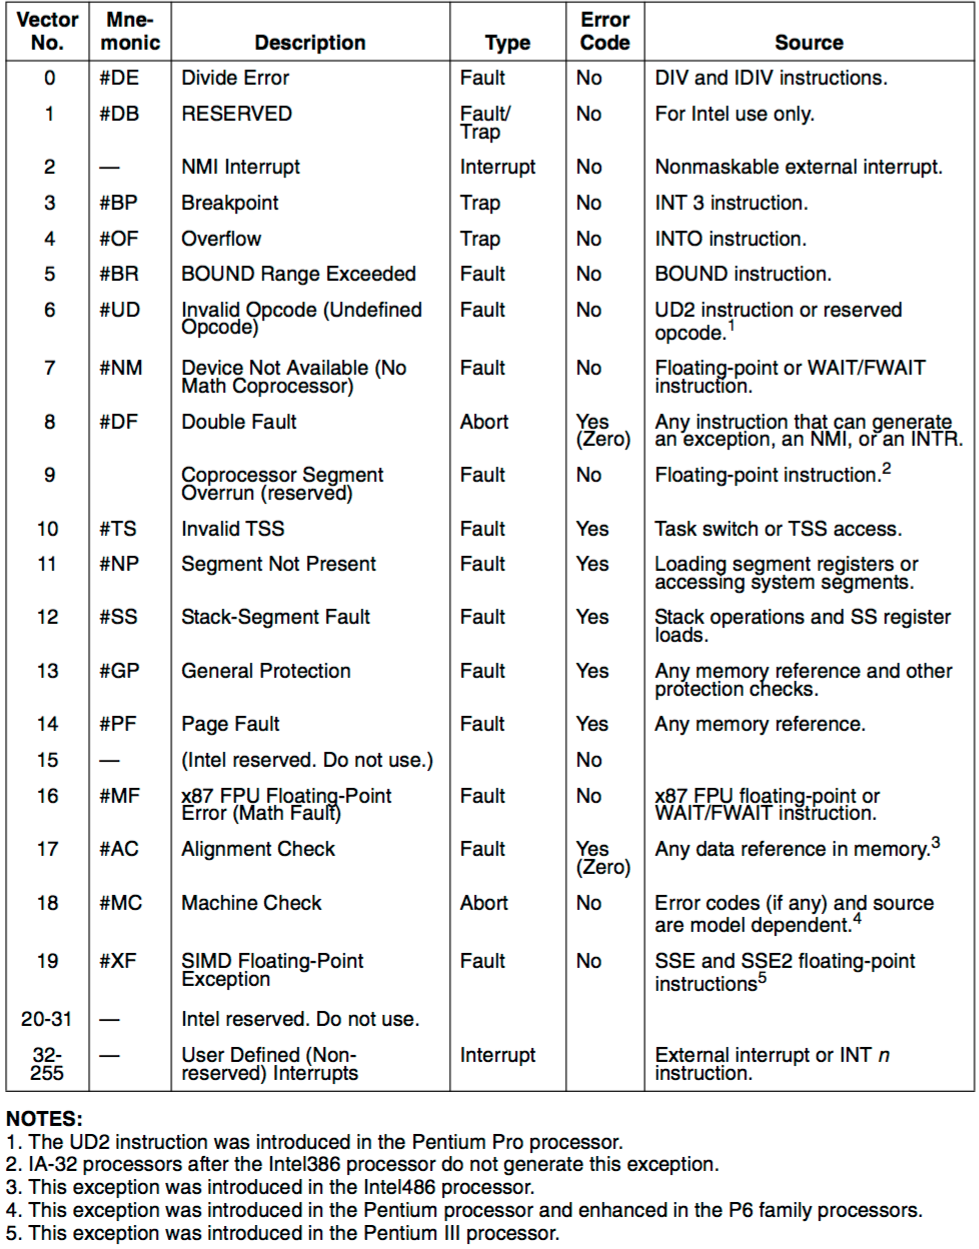
\includegraphics[scale=0.39]{images/table_int_exc.png}
  \caption{Table des interruptions et exceptions sur \acrshort{IA-32}}
  \label{table_int_exc}
\end{figure}

Comme vu précedemment, une interruption logicielle peut être exécutée par le
processeur avec l'instruction \mintinline{text}{INT}. L'instruction \mintinline{text}{INT}
suivie du numéro d'interruption sur 8 bits déclenchera l'interruption en question.
Par exemple, l'instruction \mintinline{text}{INT 0x30} déclenchera l'interruption
48. Au moment de l'appel à l'instruction \mintinline{text}{INT}, le pointeur
d'instruction va sauter à l'adresse du code contennant la routine d'interruption
correspondant au numéro d'interruption logicielle specifiée. C'est la table des
descripteurs d'interruption (\acrshort{idt}) qui permet de définir l'adresse du
code à exécuter pour chaque numéro d'interruption (que ce soit une interruption
logicielle, matérielle ou une exception). A noter aussi que les interruptions
logicielles sont synchrone étant donné qu'elles sont exécutées par le processeur,
contrairement aux interruptions matérielles qui sont asynchrones (exécutées par
les périphériques, elle peuvent arriver à n'importe quel moment). \\

Nous avons vu que les interruptions matérielles étaient générées par le \textit{hardware}.
Il existe deux types d'interruptions matérielles, les \acrshort{nmi} (\textit{Non Maskable
Interrupt}) et les \acrshort{irq} (Interrupt Request). Une \acrshort{nmi} indique
qu'un problème est survenu au niveau matériel (mémoire défectueuse, erreur de bus, ...).
Comme son nom l'indique, une \acrshort{nmi} ne peut pas être ignorée (ou masquée),
l'interruption doit donc dans tous les cas être servie. Le but ici est d'arrêter
le processeur afin d'éviter toute perte de données.\cite{ref42} Une \acrshort{irq}
quant à elle peut être masquée. L'instruction \mintinline{text}{CLI} permet de masquer
les interruptions et l'instruction \mintinline{text}{STI} permet de les démasquer.
En général, un périphérique génère une \acrshort{irq} lorsque des données sont
prêtes à être lues, qu'une commande est terminée ou qu'un évenement particulier
a lieu (par exemple la pression d'une touche du clavier ou l'écriture de données
sur le disque). Quand une interruption est générée, l'\acrshort{isr} correspondant
à l'\acrshort{irq} doit être appelée. C'est là qu'entre en jeu le controlleur
d'interruption (\acrshort{pic}). Le \acrshort{pic} va faire correspondre une
\acrshort{irq} à un numéro d'interruption (voir figure \ref{irqs}). A la manière des
interruptions logicielles l'\acrshort{idt} va être utilisée pour appeler la bonne
routine d'interruption. Le \acrshort{pic} permet donc de faire le lien entre le
matériel et le logiciel. \\

\begin{figure}[!h]
  \centering
  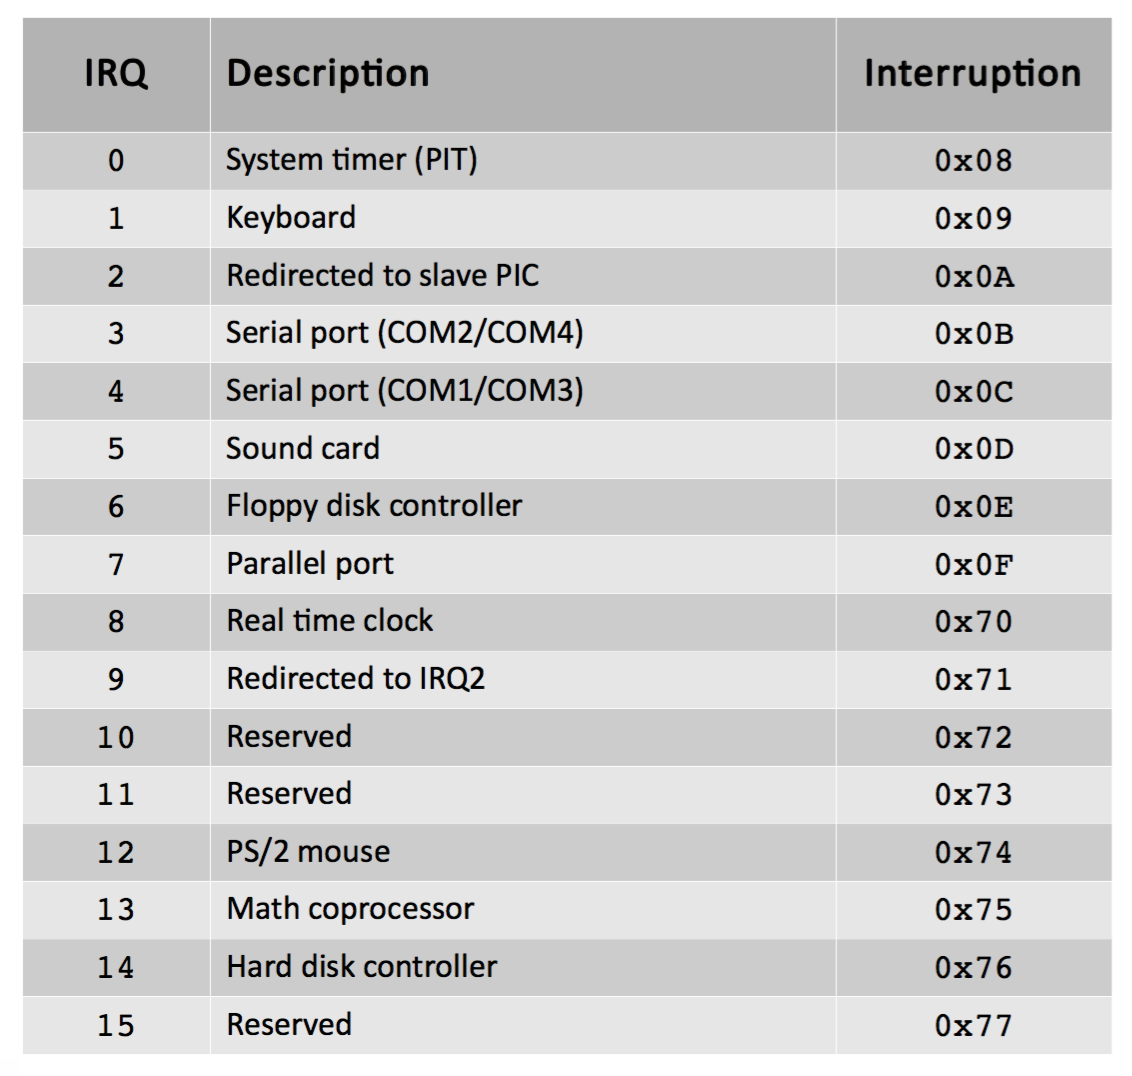
\includegraphics[scale=0.5]{images/irqs.png}
  \caption{Table de correspondance des \acrshort{irq}s}
  \label{irqs}
\end{figure}

En comparant la figure \ref{table_int_exc} avec la figure \ref{irqs}, on constate
que certaines \acrshort{irq}s partagent le même numéro d'interruption que des
exceptions. L'interruption du \textit{timer} par exemple a le même numéro d'interruption
que l'exception \textit{Double Fault} (0x8). Si on laisse le \textit{mapping} par
défaut, une interruption du \textit{timer} va déclencher une \textit{Double Fault}
ce qui n'est pas souhaitable. Il a donc été nécessaire de changer cette table
de correspondance. Les \acrshort{irq}s 0 à 7 ont été associées aux interruptions
32 à 39 et les \acrshort{irq}s 8 à 15 ont été associées aux interruptions 40 à 47.
Ce changement de \textit{mapping} peut se faire assez simplement en assembleur en
utilisant les ports des deux \acrshort{pic}s utilisés par les \acrshort{irq}s.
Un code d'exemple est donné sur le site OSDev.\cite{ref22}

%%%%%%%%%%%%%%%%%%%%%%%%%%%%%%%%%%%%%%%%%%%%%%%%%%%%%%%%%%%%%%%%%%

\subsubsection{\acrshort{idt}}
La table des descripteurs d'interruption (ou \acrshort{idt}) est similaire à la
\acrshort{gdt} (la table des descripteurs globaux). Elle est aussi composée de
descripteurs de 64-bits permettant chacun de référencer une interruption. Un
descripteur est composé d'un offset indiquant l'adresse de l'\acrshort{isr} (la
routine d'interruption), un selecteur de segment indiquant le segment où se trouve
le code de l'\acrshort{isr} et un niveau de privilège indiquant le niveau de privilège
requis pour exécuter l'\acrshort{isr}. Dans le cas d'un adressage de type \textit{FLAT}
comme celui utilisé, le selecteur de segment sera forcément le selecteur de segment
de code. Il existe aussi plusieurs types de descripteurs d'interruptions\cite{ref66}
décrits dans la figure \ref{idt_entry}. Dans le cas de notre \textit{kernel} seulement
deux types ont été utilisés, le type \textit{Interrupt Gate} et le type \textit{Trap Gate}.
La différence entre un \textit{Interrupt Gate} et un \textit{Trap Gate} est uniquement
le comportement du \acrshort{cpu} lors de l'exécution de l'\acrshort{isr}\cite{ref42}.
Dans le cas du \textit{Interrupt Gate}, le \acrshort{cpu} masquera les interruptions
lors de l'exécution de l'\acrshort{isr} alors que dans un \textit{Trap Gate} ce
ne sera pas le cas. \\

\begin{figure}[!h]
  \centering
  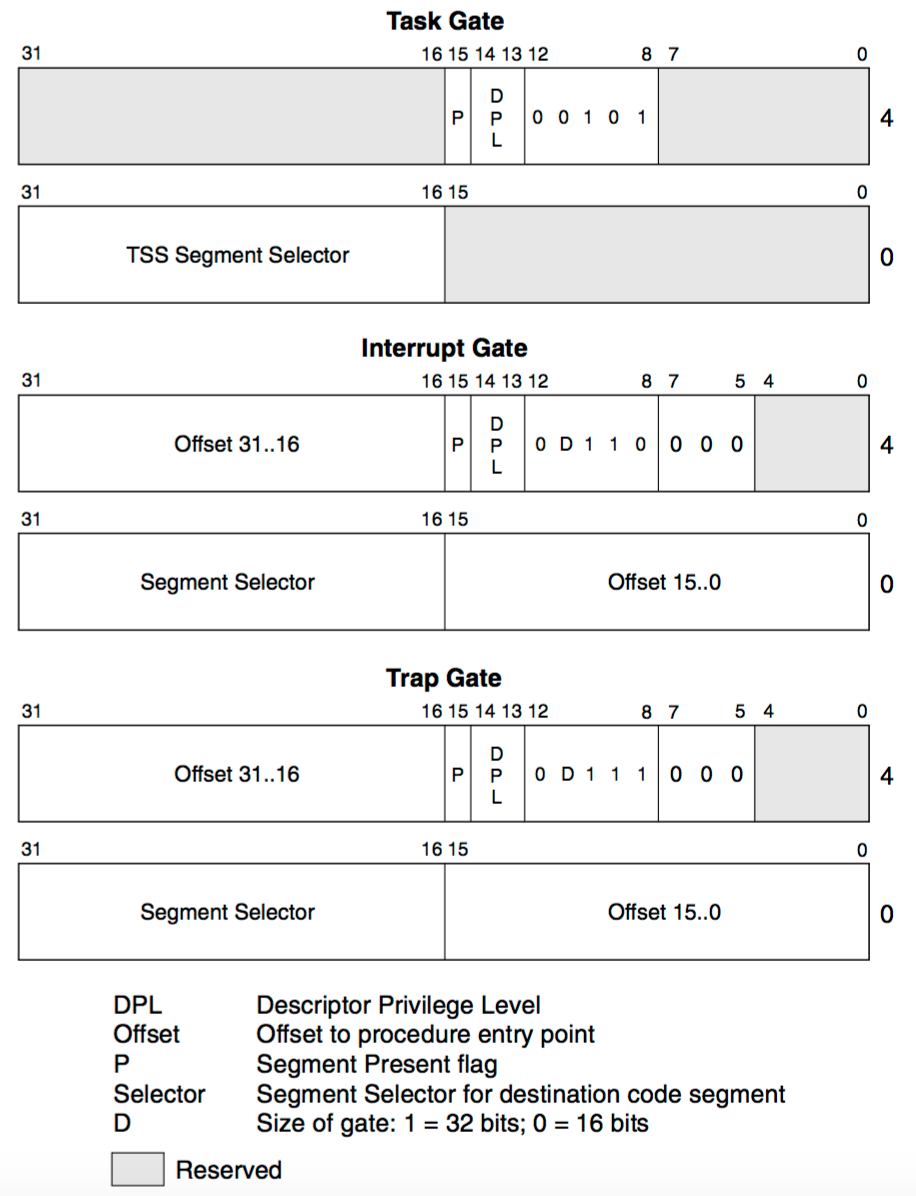
\includegraphics[scale=0.75]{images/idt_entry.png}
  \caption{Différents types de descripteur d'interruption}
  \label{idt_entry}
\end{figure}

Comme pour la \acrshort{gdt}, l'\acrshort{idt} est stockée en \acrshort{ram}
et doit donc être initialisée et gérée par l'\acrshort{os}. De la même manière
que l'instruction \mintinline{text}{LGDT} permet de charger la \acrshort{gdt},
l'instruction \mintinline{text}{LIDT} permet de charger l'\acrshort{idt} dans le
registre IDTR. Pour se faire il faut donner comme argument à l'instruction 
\mintinline{text}{LIDT} l'adresse du descripteur d'\acrshort{idt} sur 48 bits.
Ce descripteur est composé de l'adresse de l'\acrshort{idt} sur 32 bits et de sa
limite (sa taille en bytes - 1) sur 16 bits. Une fois la table des descripteurs
d'interruption chargée avec l'instruction \mintinline{text}{LIDT}, les interruptions
peuvent être activées en utilisant l'instruction \mintinline{text}{STI}. La figure
\ref{idtr} permet de résumer la relation entre le registre IDTR et l'\acrshort{idt}.

\begin{figure}[!h]
  \centering
  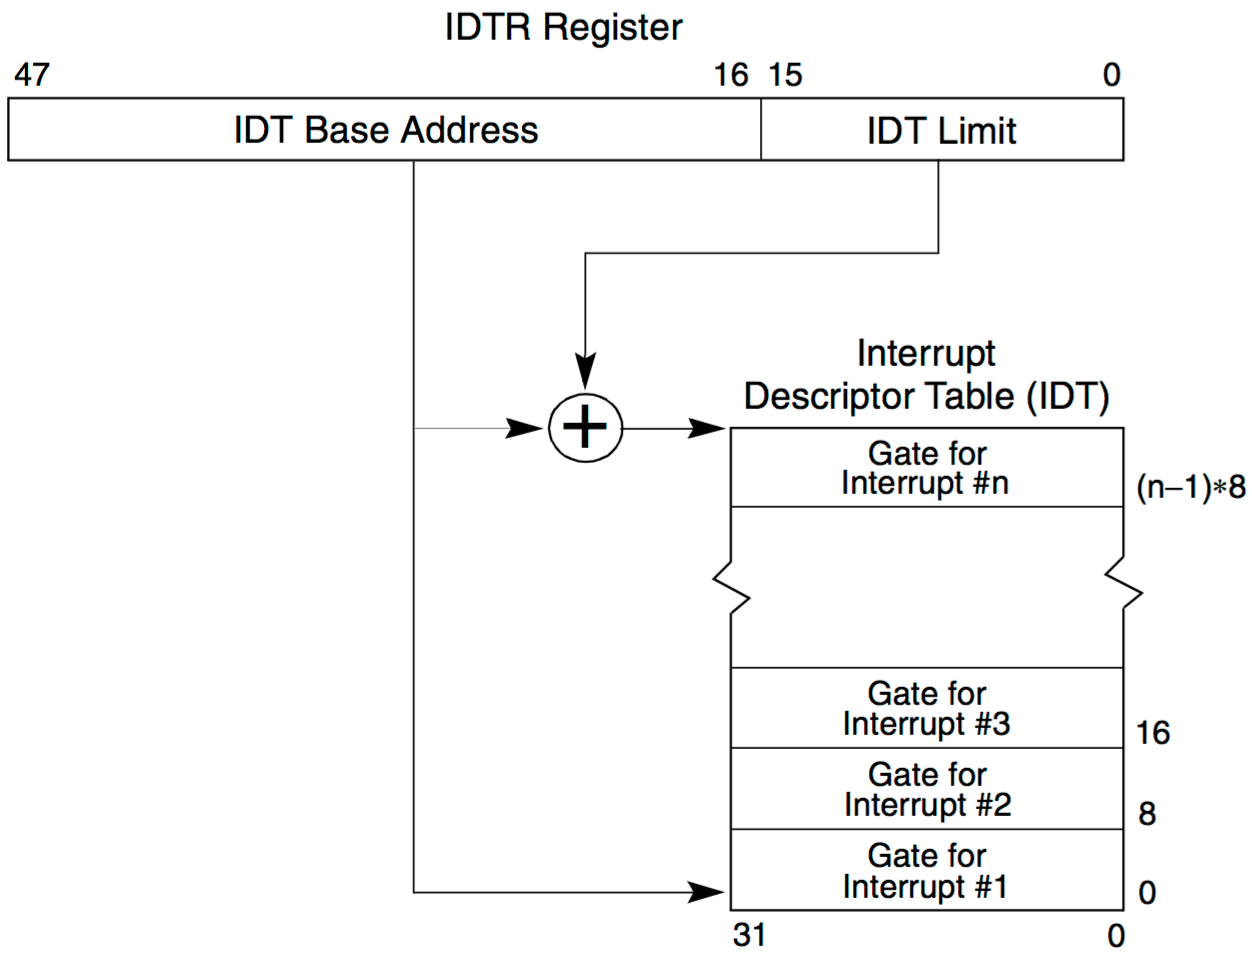
\includegraphics[scale=0.6]{images/idtr.png}
  \caption{Relation entre le registre IDTR et l'\acrshort{idt}}
  \label{idtr}
\end{figure}

Dans le \textit{kernel} développé, l'\acrshort{idt} est une structure statique
en mémoire. Une fonction assembleur est donc appelée afin de charger cette
structure dans le registre IDTR. En plus du chargement de l'\acrshort{idt}, une
partie des routines d'interruptions est faite en assembleur. En effet, il a été
nécéssaire de passer par du code bas niveau car avant de rentrer dans une
routine d'interruption, il faut sauvegarder le contexte. Il est obligatoire
de sauvegarder le contexte car, comme déjà dit plus haut, une interruption
peut avoir lieu à n'importe quel moment. La partie bas niveau de la routine
d'interruption s'occupe donc de sauvegarder le contexte puis d'appeler un
gestionnaire d'interruption haut niveau en rust. Ce gestionnaire prend comme argument
le numéro d'interruption et appelle la routine d'interruption liée à cette interruption.
Par exemple, la routine d'interruption du \textit{timer} va simplement incrémenter
un compteur. Lorsque une exception est levée le même mécanisme est employé sauf
qu'ici le \textit{kernel} va afficher un message d'erreur en fonction du numéro
de l'exception.

%%%%%%%%%%%%%%%%%%%%%%%%%%%%%%%%%%%%%%%%%%%%%%%%%%%%%%%%%%%%%%%%%%
%%%%%%%%%%%%%%%%%%%%%%%%%%%%%%%%%%%%%%%%%%%%%%%%%%%%%%%%%%%%%%%%%%

\subsection{\acrshort{vga}}
Dans l'\acrshort{os} développé, le mode texte \acrshort{vga} a été utilisé pour
l'affichage. Toute carte graphique offre ce mode texte de 80 colonnes par 25 lignes.
Les 16 couleurs disponibles sont les suivantes :\cite{ref19}
\begin{figure}[!h]
  \centering
  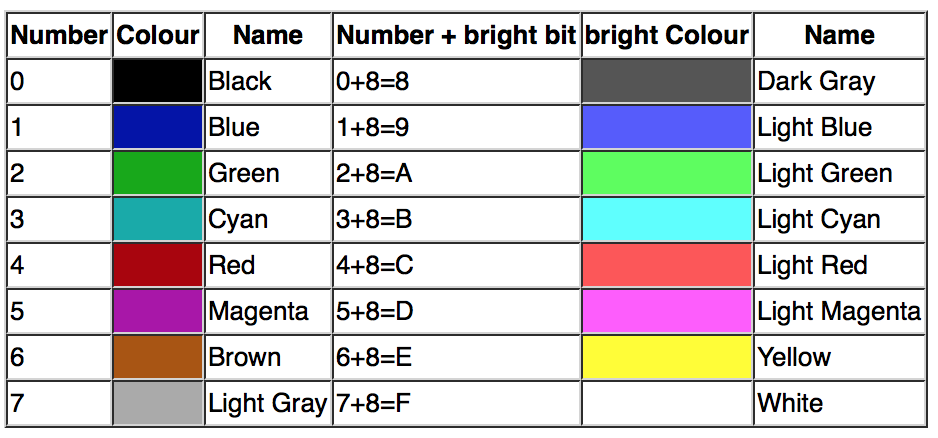
\includegraphics[scale=0.7]{images/colors.png}
  \caption{Couleurs du mode texte \acrshort{vga}}
\end{figure}

%%%%%%%%%%%%%%%%%%%%%%%%%%%%%%%%%%%%%%%%%%%%%%%%%%%%%%%%%%%%%%%%%%
%%%%%%%%%%%%%%%%%%%%%%%%%%%%%%%%%%%%%%%%%%%%%%%%%%%%%%%%%%%%%%%%%%

\subsection{\textit{Timer}}

%%%%%%%%%%%%%%%%%%%%%%%%%%%%%%%%%%%%%%%%%%%%%%%%%%%%%%%%%%%%%%%%%%
%%%%%%%%%%%%%%%%%%%%%%%%%%%%%%%%%%%%%%%%%%%%%%%%%%%%%%%%%%%%%%%%%%

\subsection{Clavier}